
Kelompok : 4
Kelas : D4 TI 1A
Anggota : 
1. Damara Benedikta		1174012
2. Duvan Silalahi 		1174011
3. Ilham Habibi			1174028
4. Muhammad Fahmi		1174021
5. Oniwaldus Bere mali	1174005


\section Sistem Paging
Sistem Paging Adalah sistem manajemen pada sistem operasi dalam mengatur program yang sedang berjalan. Program yang berjalan harus dimuat di memori utama. Kendala yang terjadi apabila suatu program lebih besar dibandingkan dengan memori utama yang tersedia.

Untuk mengatasi hal tersebut Sistem Paging mempunyai 2 solusi, yaitu:

\subsection Konsep Overlay
Dimana program yang dijalankan dipecah menjadi beberapa bagian yang dapat dimuat memori (overlay). Overlay yang belum diperlukan pada saat program berjalan (tidak sedang di eksekusi) disimpan di disk, dimana nantinya overlay tersebut akan dimuat ke memori begitu diperlukan dalam eksekusinya.

Konsep Memori Maya (virtual Memory)
Adalah kemampuan mengalamati ruang memori melebihi memori utama yang tersedia. Konsep ini pertama kali dikemukakan Fotheringham pada tahun 1961 untuk sistem komputer Atlas di Universitas Manchester, Inggris \ref{Gambar1}.

Gagasan Memori Maya adalah ukuran gabungan program, data dan stack melampaui jumlah memori fisik yang tersedia. Sistem operasi menyimpan bagian-bagian proses yang sedang digunakan di memori utama dan sisanya di disk. Begitu bagian di disk diperlukan maka bagian memori yang tidak diperlukan disingkirkan dan diganti bagian disk yang diperlukan.


	\begin{figure}[ht]
	\centerline{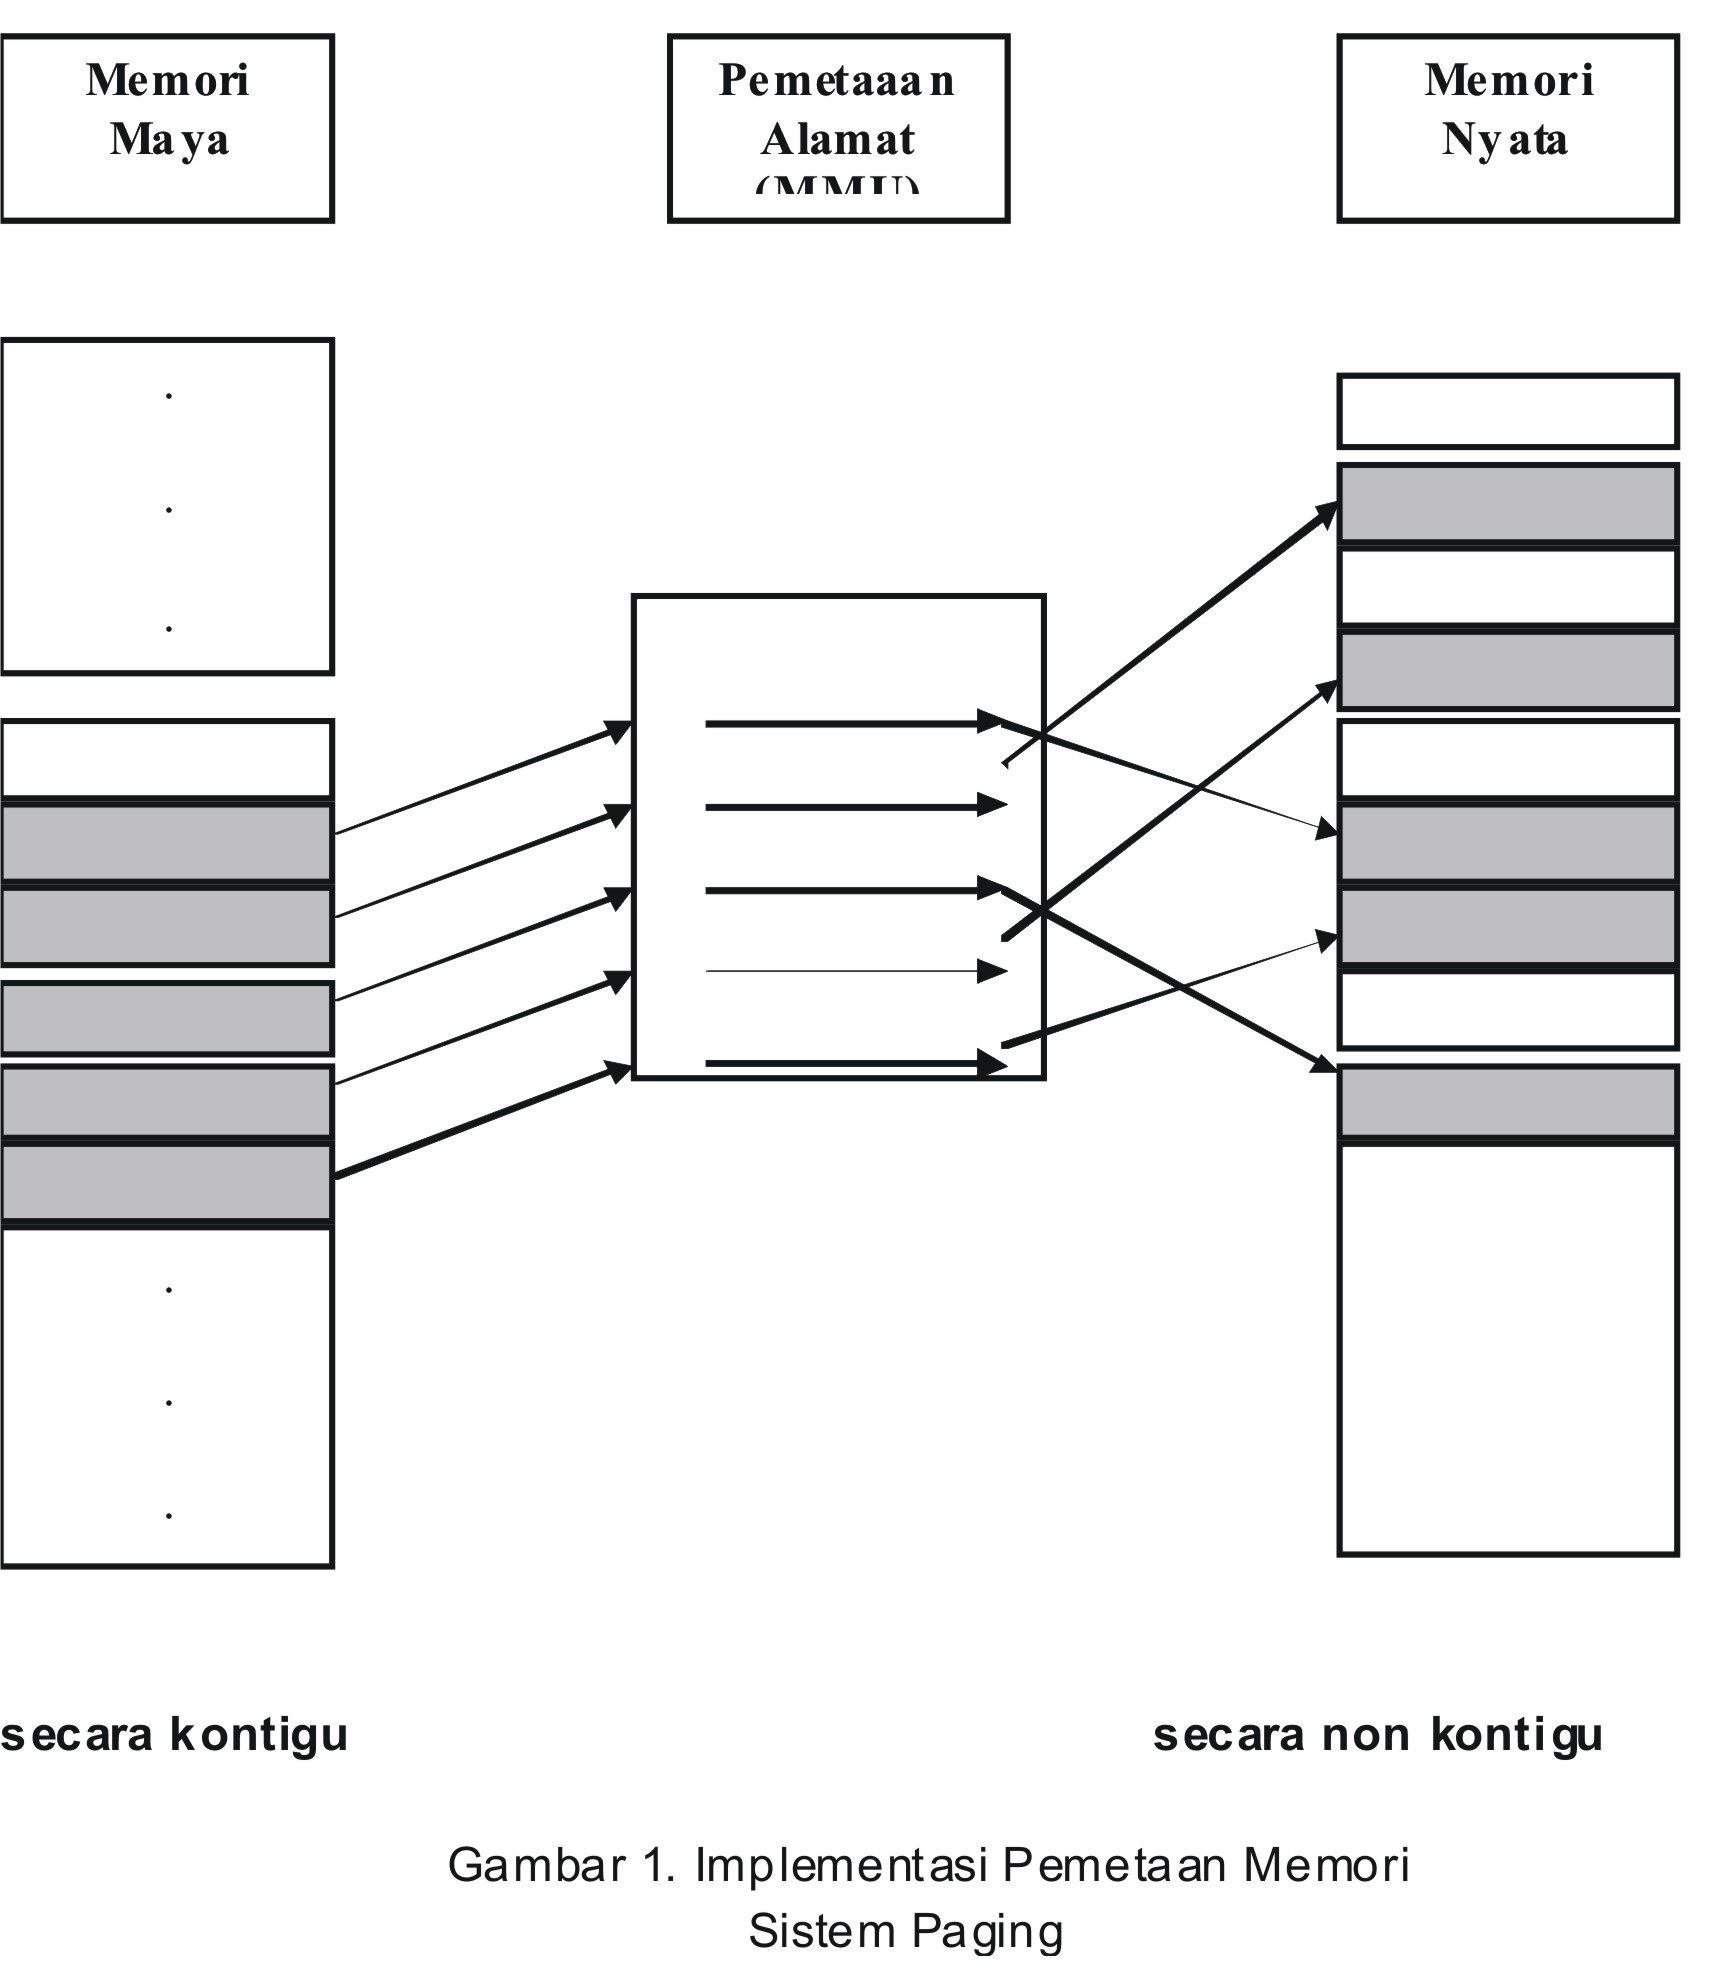
\includegraphics[width=1\textwidth]{figures/gambarpaging1.jpg}}
	\caption{Implementasi pemetaan memori system paging.}
	\label{Gambar1}
	\end{figure}

\section Masalah Penggantian Halaman

Berdasarkan pertimbangan tersebut, sebenarnya proses-proses yang memiliki 10 halaman hanya akan menggunakan setengah dari jumlah seluruh halaman yang dimilikinya. Kemudian demand paging akan menyimpan I/O yang dibutuhkan untuk mengisi 5 halaman yang belum pernah digunakan. Kita juga dapat meningkatkan derajat multiprogramming dengan menjalankan banyak proses sebanyak 2 kali.

\section sistem paging 
pengertian sistem paging 
Sistem Paging Merupakan sistem yang memanajemen pada sistem operasi dalam mengelola program program yang sedang berjalan. Program program yang berjalan harus dimuat didalam memori utama. Batasan batasan yang terjadi saat program lebih besar dari memori utama yang telah tersedia. 
\cite{Fomukong}.

\subsection pembagian solusi sistem paging 
a.Konsep Overlay
b.Konsep Memori Maya (virtual Memory)


\section Masalah Penggantian Halaman 
 
Pada dasarnya, kesalahan halaman (page fault) sudah tidak lagi menjadi masalah yang terlalu  dianggap serius. Hal ini disebabkan karena masing-masing halaman pasti akan mengalami paling tidak satu kali kesalahan dalam pemberian halaman, yakni ketika halaman ini ditunjuk untuk pertama kalinya. Representasi seperti ini sebenarnya tidaklah terlalu akurat. 
=======
a. Konsep Overlay
Dimana program yang dijalankan dipecah menjadi beberapa bagian yang dapat dimuat memori (overlay). Overlay yang belum diperlukan pada saat program berjalan (tidak sedang di eksekusi) disimpan di disk, dimana nantinya overlay tersebut akan dimuat ke memori begitu diperlukan dalam eksekusinya.

b. Konsep Memori Maya (virtual Memory)
Adalah kemampuan mengalamati ruang memori melebihi memori utama yang tersedia. Konsep ini pertama kali dikemukakan Fotheringham pada tahun 1961 untuk sistem komputer Atlas di Universitas Manchester, Inggris.

\section penggantian halaman
Pada dasarnya, kesalahan halaman tidak lagi menjadi masalah serius. Ini karena setiap halaman akan mengalami setidaknya satu kesalahan dalam pengiriman halaman, yaitu ketika halaman ini ditujukan untuk pertama kalinya. Representasi seperti ini sebenarnya tidak terlalu akurat. Berdasarkan pertimbangan ini, sebenarnya proses yang memiliki 10 halaman hanya akan menggunakan setengah dari jumlah total halaman yang dimilikinya. Kemudian permintaan paging akan menyimpan I / O yang diperlukan untuk mengisi 5 halaman yang belum pernah digunakan. Kami juga dapat meningkatkan tingkat multiprogramming dengan menjalankan beberapa proses 2 kali.

Lebih jauh lagi, kita harus mempertimbangkan bahwa sistem memori tidak hanya digunakan untuk menangani pengalamatan suatu program. Penyangga (buffer) untuk I/O juga menggunakan sejumlah memori. Penggunaan ini dapat meningkatkan pemakaian algoritma dalam penempatan di memori.

Beberapa sistem mengalokasikan secara pasti beberapa persen dari memori yang dimilikinya untuk penyangga I/O, dimana keduanya, baik proses

Lebih jauh lagi, kita harus mempertimbangkan bahwa sistem memori tidak hanya digunakan untuk menangani pengalamatan suatu program. Buffer untuk I / O juga menggunakan beberapa memori. Penggunaan ini dapat meningkatkan penggunaan algoritma dalam penempatan di memori.
Beberapa sistem mengalokasikan persis beberapa persen dari memori mereka untuk menyangga I / O, di mana keduanya,


Beberapa sistem mengalokasikan tepat beberapa persen dari memori mereka untuk buffer I / O, keduanya, baik proses pengguna dan subsistem I / O race untuk mengambil keuntungan dari seluruh sistem memori.

\section skema dasar pemindahan halaman 
Pemindahan halaman menggunakan pendekatan berikut. Jika tidak ada frame yang kosong, kami mencari frame yang tidak digunakan dan mengosongkannya. Kita dapat mengosongkan bingkai dengan menulis isinya ke dalam ruang swap, dan mengubah tabel halaman (serta tabel lainnya) untuk menunjukkan bahwa halaman tidak akan lama dalam memori.


\subsection cara memindahkan halaman

\begin{table}[H]
\begin{tabular}{|c|c|c|c|c|}
hline
No. & Nama & Jenis Kelamin & Pekerjaan & Alamat\\
\hline
1   & Cari lokasi dari halaman yang diinginkan pada disk
 & & &\\
2   & Cari frame kosong
 & & &\\
3   & Baca halaman yang diinginkan kedalam frame kosong yang baru & & &\\
4   & Ulang dari awal proses pengguna. & &\\
\hline
\end{tabular}
\end{table}

1. Cari lokasi dari halaman yang diinginkan pada disk

2. Cari frame kosong

a. Jika ada frame kosong, gunakan.
b. Jika tidak ada frame kosong, gunakan algoritma pemindahan halaman untuk menyeleksi frame yang akan digunakan.
c. Tulis halaman yang telah dipilih ke disk, ubah tabel halaman dan tabel frame.

3. Baca halaman yang diinginkan kedalam frame kosong yang baru, ubah tabel halaman dan tabel frame
 
4. Ulang dari awal proses pengguna.

Kita harus menyelesaikan 2 masalah utama untuk mengimplementasikan demand paging. Kita harus  mengembangkan algoritma pengalokasian rame dan algoritma pemindahan halaman. Jika kita memiliki banyak proses di memori, kita harus memutuskan berapa banyak frame yang akan dialokasikan ke masing-masing proses. Lebih jauh lagi, saat pemindahan halaman diinginkan, kita harus memilih frame yang akan dipindahkan. Membuat suatu algoritma yang tepat untuk menyelesaikan masalah ini adalah hal yang sangat penting.
ini adalah hal yang sangat penting.

Ada beberapa algoritma pemindahan halaman yang berbeda. Kemungkinan setiap Sistem Operasi memiliki skema pemindahan yang unik. Algoritma pemindahan yang baik adalah yang memiliki tingkat kesalahan halaman terendah. Kita mengevaluasi algoritma dengan menjalankanny dalam string khusus di memori acuan dan menghitung jumlah kesalahan halaman.  String dari memori acuan disebut string acuan (reference string). Sebagai contoh, jika kita memeriksa proses khusus, kita mungkin akan mencatat urutan alamat seperti dibawah ini:
0100, 0432, 0101, 0612, 0102, 0103, 0104, 0101, 0611, 0102, 0103, 0104, 0101, 0610, 0102, 0103,

0104, 0101, 0609, 0102, 0105, di mana pada 100 byte per halaman, diturunkan menjadi string referensi sebagai berikut:

1, 4, 1, 6, 1, 6, 1, 6, 1, 6, 1 

Perhatikan bahwa selama jumlah frame meningkat, jumlah kesalahan halaman menurun.

Penambahan memori fisik akan menambah jumlah frame.

\section Pemindahan Halaman Secara FIFO

Algoritma ini adalah algoritma paling sederhana dalam hal pemindahan halaman. Algoritma pemindahan


Pemindahan Halaman Secara FIFO

Algoritma ini adalah algoritma paling sederhana dalam hal pemindahan halaman. Algoritma pemindahan


Sebagai contoh:
Gambar 4-11. String Acuan. Sumber: . . .

7 0 1 2 0 3 0 4 2 3 0 3 2 1 2 0 1 7 0 1

7 7 7 2 2 2 4 4 4 0 0 0 7 7 7

0 0 0 3 3 3 2 2 2 1 1 1 0 0

1 1 1 0 0 0 3 3 3 2 2 2 1

Dari contoh contoh di atas, ada 15 halaman kesalahan. Algoritma FIFO mudah dimengerti dan diimplementasikan. Namun kinerjanya tidak selalu baik. Salah satu kelemahan dari algoritma FIFO adalah kemungkinan anomali Beladi, yang ada dalam beberapa kasus, tingkat kesalahan akan meningkat apabila jumlah frame yang dialokasikan juga meningkat.

\section pemindahan halaman secara optimal 
Salah satu konsekuensi mencegah anomali Beladi adalah algoritma pergerakan halaman yang optimal. Algoritma ini memiliki tingkat kesalahan halaman terendah dibandingkan dengan algoritma lainnya. Algoritma ini tidak akan mengalami anomali Belady. Konsep utama dari algoritma ini adalah mengganti halaman yang tidak akan digunakan untuk periode waktu terlama. Algoritma ini memastikan tingkat kesalahan serendah mungkin untuk sejumlah frame yang tetap.

\subsection Perlu disayangkan, algoritma optimal susah untuk diimplementasikan kedalam program, karena algoritma ini menuntut pengetahuan tentang string acuan yang akan muncul.

\section Pemindahan Halaman Secara LRU

Jika algoritma optimal sulit untuk dilakukan, mungkin kita dapat melakukan pendekatan terhadap algoritma tersebut. Jika kita menggunakan waktu yang baru berlalu sebagai pendekatan terhadap waktu yang akan datang, 

\subsection
(Least Recently Used) Rekan algoritma LRU dengan setiap halaman waktu dari halaman yang terakhir digunakan. Ketika halaman harus dipindahkan, LRU memilih halaman terpakai terpanjang di masa lalu. Berikut adalah algoritma LRU, lihat waktu lampau, bukan waktu yang akan datang.

Untuk mengimplementasikan algoritma LRU, ada 2 implementasi yang dapat digunakan, yaitu dengan counter dan stack. Selain algoritma optimal, algoritma LRU juga dapat menghindari anomali Beladi. Salah satu kelas algoritma halaman bergerak adalah algoritma tumpukan, yang juga tidak akan pernah mengalami anomali Beladi. Algoritma tumpukan ini menyimpan nomor halaman pada tumpukan. Kapan pun suatu halaman ditunjuk, halaman ini dikeluarkan dari tumpukan dan diletakkan di blok paling atas dari tumpukan. Dengan cara seperti ini, blok paling atas dari tumpukan selalu berisi halaman yang baru digunakan, sedangkan blok terbawah dari tumpukan selalu berisi halaman yang sudah lama tidak digunakan. Karena suatu halaman dalam tumpukan dapat dikeluarkan meski pun berada ditengah-tengah meski pun berada ditengah-tengah stack, maka implementasi terbaik untuk algoritma ini adalah dengan daftar mata rantai ganda ( doubly linked list), dengan kepala dan ekor sebagai penunjuk. Pendekatan ini sangat tepat untuk perangkat lunak atau implementasi kode mikro dari algoritma LRU.
 
\section Pemindahan Halaman Secara Perkiraan LRU

Awalnya, semua bit dikosongkan oleh sistem operasi. Selama proses pengguna, bit-bit yang terkait dengan setiap halaman referensi diatur ke 1 oleh perangkat keras. Setelah beberapa waktu, kami dapat menentukan halaman mana yang telah digunakan dan halaman mana yang belum digunakan dengan menguji bit referensi. Informasi ini memberikan informasi penting bagi banyak algoritma pemindahan halaman yang memperkirakan halaman mana yang tidak digunakan untuk waktu yang lama.
 
\section Algoritma Additional-Reference-Bit

Kita bisa mendapatkan informasi tambahan mengenai urutan dengan mencatat bit-bit acuan pada suatu interval yang tetap. Kita dapat menyimpan 8-bit byte untuk masing-masing halaman pada tabel di memori. Pada interval tertentu, pencatat waktu (timer) melakukan interupsi dengan mentransfer kontrol kepada sistem operasi. Sistem operasi mengubah bit acuan untuk masing-masing halaman kedalam bit high-order dari 8-bit byte ini dan membuang bit low-order. Register pengganti 8-bit ini berisi sejarah penggunaan halaman dalam periode 8 waktu terakhir.Sebagai contoh, seandainya register pengganti berisi 00000000, maka itu berarti halaman sudah tidak digunakan dalam periode 8 waktu terakhir, halaman yang digunakan paling tidak 1 kali akan memiliki nilai register penggati 11111111.

\section Algoritma second-chance
Algoritma second-chance didasarkan pada algoritma FIFO. Ketika sebuah halaman diarahkan, kita akan memeriksa bit referensi jika bit referensi adalah 0, kita memproses untuk menghapus halaman ini. Jika bit referensi adalah 1, kita memberikan kesempatan kedua. untuk halaman ini dan pilih halaman FIFO berikutnya.

Ketika halaman mendapat kesempatan kedua, bit referensi-nya akan dihapus dan waktu di-reset ke arus. Oleh karena itu, halaman yang mendapat kesempatan kedua tidak akan
dipindahkan sampai seluruh halaman dipindahkan. Selain itu, jika halaman yang digunakan cukup untuk menampung 1 set bit referensi, maka halaman ini tidak akan pernah dipindahkan.

\section Algoritme Second-Chance (Fixed)

Kita dapat memperbaiki kekurangan dari algoritma kesempatan kedua dengan mempertimbangkan 2 hal
sekaligus, bit referensi dan bit yang dimodifikasi. Dengan 2 bit ini, kita akan mendapatkan 4 kemungkinan
yang akan terjadi, yaitu:
• (0,0) tidak terpakai dan tidak dimodifikasi, sedikit terbaik untuk bergerak.

• (0,1) tidak digunakan tetapi dimodifikasi, tidak terlalu bagus untuk dipindahkan karena halaman ini perlu ditulis sebelum dipindahkan.

• (1.0) digunakan tetapi tidak dimodifikasi, mungkin halaman ini akan digunakan lagi segera.
 
• (1,1) digunakan dan dimodifikasi, halaman ini dapat segera digunakan lagi dan halaman ini harus ditulis ke disk sebelum dipindahkan. Algoritma ini digunakan dalam skema manajemen memori virtual Macintosh.
